%% For double-blind review submission, w/o CCS and ACM Reference (max submission space)
\documentclass[acmsmall,anonymous,review]{acmart}\settopmatter{printfolios=true,printccs=false,printacmref=false}
%% For double-blind review submission, w/ CCS and ACM Reference
%\documentclass[sigplan,10pt,review,anonymous]{acmart}\settopmatter{printfolios=true}
%% For single-blind review submission, w/o CCS and ACM Reference (max submission space)
%\documentclass[sigplan,10pt,review]{acmart}\settopmatter{printfolios=true,printccs=false,printacmref=false}
%% For single-blind review submission, w/ CCS and ACM Reference
%\documentclass[sigplan,10pt,review]{acmart}\settopmatter{printfolios=true}
%% For final camera-ready submission, w/ required CCS and ACM Reference
%\documentclass[sigplan,10pt]{acmart}\settopmatter{}

%% Conference information
%% Supplied to authors by publisher for camera-ready submission;
%% use defaults for review submission.
\acmConference[PL'18]{ACM SIGPLAN Conference on Programming Languages}{January 01--03, 2018}{New York, NY, USA}
\acmYear{2018}
\acmISBN{} % \acmISBN{978-x-xxxx-xxxx-x/YY/MM}
\acmDOI{} % \acmDOI{10.1145/nnnnnnn.nnnnnnn}
\startPage{1}

%% Copyright information
%% Supplied to authors (based on authors' rights management selection;
%% see authors.acm.org) by publisher for camera-ready submission;
%% use 'none' for review submission.
\setcopyright{none}
%\setcopyright{acmcopyright}
%\setcopyright{acmlicensed}
%\setcopyright{rightsretained}
%\copyrightyear{2017}           %% If different from \acmYear

%% Bibliography style
\bibliographystyle{ACM-Reference-Format}
%% Citation style
%\citestyle{acmauthoryear}  %% For author/year citations
%\citestyle{acmnumeric}     %% For numeric citations
%\setcitestyle{nosort}      %% With 'acmnumeric', to disable automatic
                            %% sorting of references within a single citation;
                            %% e.g., \cite{Smith99,Carpenter05,Baker12}
                            %% rendered as [14,5,2] rather than [2,5,14].
%\setcitesyle{nocompress}   %% With 'acmnumeric', to disable automatic
                            %% compression of sequential references within a
                            %% single citation;
                            %% e.g., \cite{Baker12,Baker14,Baker16}
                            %% rendered as [2,3,4] rather than [2-4].


\usepackage{graphicx}
\usepackage{subfig}
\usepackage{caption}
%\usepackage{subcaption}
\usepackage[export]{adjustbox}

\begin{document}

% \newcommand{\charcoal}{Charcoal}
\newcommand{\charcoal}{DblBlind}
\newcommand{\atomic}{\texttt{atomic}}

\special{papersize=8.5in,11in}
\setlength{\pdfpageheight}{\paperheight}
\setlength{\pdfpagewidth}{\paperwidth}

% \titlebanner{Preprint.  Please do not redistribute}        % These are ignored unless
% \preprintfooter{Preprint.  Please do not redistribute}   % 'preprint' option specified.

\title{Atomicity in Cooperative Concurrency: Measurements, Language Design and Implementation}
% \subtitle{\ldots and How to Make Cooperative Concurrency Safer with \texttt{atomic}}

%% Author information
%% Contents and number of authors suppressed with 'anonymous'.
%% Each author should be introduced by \author, followed by
%% \authornote (optional), \orcid (optional), \affiliation, and
%% \email.
%% An author may have multiple affiliations and/or emails; repeat the
%% appropriate command.
%% Many elements are not rendered, but should be provided for metadata
%% extraction tools.

%% Author with single affiliation.
\author{Benjamin Ylvisaker}
% \authornote{with author1 note}          %% \authornote is optional;
                                        %% can be repeated if necessary
% \orcid{nnnn-nnnn-nnnn-nnnn}             %% \orcid is optional
\affiliation{
  \position{Assistant Professor}
  \department{Department of Math and Computer Science}
  \institution{Colorado College}
  \streetaddress{14 E Cache La Poudre St}
  \city{Colorado Springs}
  \state{CO}
  \postcode{80903}
  \country{USA}
}
\email{bylvisaker@coloradocollege.edu}


\begin{abstract}

  ABSTRACT
%% This paper is about combining cooperative concurrency with atomic blocks.
%% In particular, we address two primary questions:
%% Why might this combination be useful?
%% What is tricky about making a clean semantics and implementation for languages that combine these concepts?

%%   The sophistication of multitasking in mainstream software has increased in recent years, thanks to the increasing richness of network communication, physical world interaction and multi-process software architectures.
%% These trends have pushed programming languages to offer better ways of writing such code.
%% As just one example of this trend, in recent years some flavor of coroutine has been standardized (or is heading towards standardization) in JavaScript, Swift, and C++.

%% This paper makes two primary contributions.
%% The first is an empirical study of multitasking in modern web applications.
%% Our primary finding is that in current practice, web JavaScript code tends to exhibit risky patterns, from the perspective of atomicity.
%% We argue that an \texttt{atomic} block primitive should be added to languages to help programmers avoid atomicity bugs.

%% We also experiment with two implementations of cooperative threads plus atomic: a JavaScript library and a dialect of C.
%% This investigation shows that this language design can be implemented in a flexible and efficient way.

\end{abstract}


%% 2012 ACM Computing Classification System (CSS) concepts
%% Generate at 'http://dl.acm.org/ccs/ccs.cfm'.
\begin{CCSXML}
<ccs2012>
<concept>
<concept_id>10011007.10011006.10011008</concept_id>
<concept_desc>Software and its engineering~General programming languages</concept_desc>
<concept_significance>500</concept_significance>
</concept>
<concept>
<concept_id>10003456.10003457.10003521.10003525</concept_id>
<concept_desc>Social and professional topics~History of programming languages</concept_desc>
<concept_significance>300</concept_significance>
</concept>
</ccs2012>
\end{CCSXML}

\ccsdesc[500]{Software and its engineering~General programming languages}
\ccsdesc[300]{Social and professional topics~History of programming languages}
%% End of generated code


%% Keywords
%% comma separated list
%% \keywords are mandatory in final camera-ready submission
\keywords{Cooperative concurrency, Multitasking, Atomicity}

\maketitle

% Outline:
% Introduction
%   Contributions
% Atomic or Interruptible?
%   On Atoms and Interrupts
%   Events
%   Cooperative Threads
%   Coroutines and Async Procedures}
%   What's Wrong with Threads?
% Activities
%   Shared Variables
%   Yield Insertion
%   Atomic
%   System Calls
%   Activities, Compared
% Implementation
%   Call Frame Allocation
%     Contiguous Allocation
%     Individual Heap Allocation
%     Split/Segmented Stacks
%     Dynamic Contiguous Stacks
%     Hot Stacking
%   Yield Implementation
%     Yield in Atomic Mode
%     Function Pointers
%     Yields
%   Asynchronous System Calls
%   Translation
%   Activities in JavaScript
% Evaluation
%   Building an App with Activities
%   Task Memory Overhead
%   Task Spawn and Switching Speed
%   Just Calling
%   Yielding
%   Microbenchmark Summary
% Related Work
%   Other Multitasking Abstractions
% Summary and Discussion



\section{Introduction}

Many modern applications are highly multitasked.
They have lots of balls in the air at the same time: network communication, queries to databases, multiple I/O modalities to monitor and manage.
Applications use a wide range of features in languages and core libraries to implement this multitasking: threads, event loops, coroutines, async functions, functional reactive programming, etc.
We briefly note that some of these features are also relevant to \emph{parallelism} (i.e. physical simultaneity), but parallelism is \emph{not} the subject of this paper or the project it describes.

Many popular application programming frameworks use some form of \emph{cooperative} multitasking, because of the fear that preemption too easily causes concurrency bugs.
While the authors of this paper are sympathetic with that fear, we remind the reader that cooperativeness only \emph{reduces} the risk of concurrency defects\footnotemark{}.
There has been much research in the last decade on cataloging, exposing, diagnosing and fixing concurrency bugs in web and mobile applications that use a cooperative concurrency model.

\footnotetext{This is similar to how garbage collection reduces, but does not eliminate, exposure to memory bugs\cite{Grossman2007}.}

An important concept related to avoiding concurrency bugs is atomicity.
This idea is nearly universal in the database world, where atomic transactions are used to collect together multiple reads and writes.
Herlihy and Moss \cite{Herlihy1993} kicked off decades of research on bringing this idea to general purpose multithreaded programming languages in the form of a block that can make an arbitrary sequence of statements appear atomic.

The idea of a \emph{general purpose} atomic block in multithreaded languages so far has seen little use outside of research labs, because of challenges with efficient implementation and elegantly handling semantic corner cases.
At the broadest scope, the question addressed in this paper is: Is it a good idea to combine atomic blocks with cooperative concurrency models, like event loops or cooperative threads?
This breaks into three primary sub-questions:
\begin{itemize}
\item Is it beneficial from a software engineering perspective to have atomic blocks in cooperative concurrency languages?
\item Are there any semantic or language design problems with this combination of features?
\item Are there interesting implementation efficiency issues raised by this combination of features?
\end{itemize}

We gather evidence for the first question by measuring widely used web applications\footnotemark{}.
We observe that patterns that seem risky from an atomicity perspective are common on the web.
In particular, there are many short-duration chains of continuations.
We believe it would be easy for a developer to test such code and effectively assume atomicity for the chain, even though it is possible for conflicting tasks to execute in a gap between continuations.

\footnotetext{We study web applications for the simple reason that a large amount of presumably high quality code is easily available for the studying.}

In investigating the second question, we noticed the following conflict with combining atomic blocks and anonymous cooperative concurrency:
\begin{enumerate}
\item There are multiple reasonable semantics for the nesting of atomic blocks and task spawns; no interpretation works well in all contexts.
\item Many cooperative concurrency frameworks are anonymous in the sense that they lack an explicit notion of task identity.
  This makes it hard to know whether an asynchronous continuation is logically a continuation of its parent task, or a new concurrent task.
  This further compounds the problem with atomic and spawn nesting, because spawns cannot be identified unambiguously.
\end{enumerate}
To the best of our knowledge, this is a novel observation.
This implies that \emph{if} a cooperative multitasking framework is to include atomic blocks, it should have explicit task identities (i.e. some flavor of cooperative threading).

To investigate the third question, we implemented cooperative threads with atomic blocks in two contexts: as a library built on top of JavaScript's async functions and as a dialect of C.
We observe that such a library can be used with modest code complexity relative to popular JavaScript patterns, and that it mostly integrates well with legacy code.
In the C dialect implementation we discover a new call frame allocation strategy -- enabled by atomic blocks -- that combines the speed benefits of contiguous frame allocation with the memory benefits of individual linked frame allocation.

\begin{figure*}
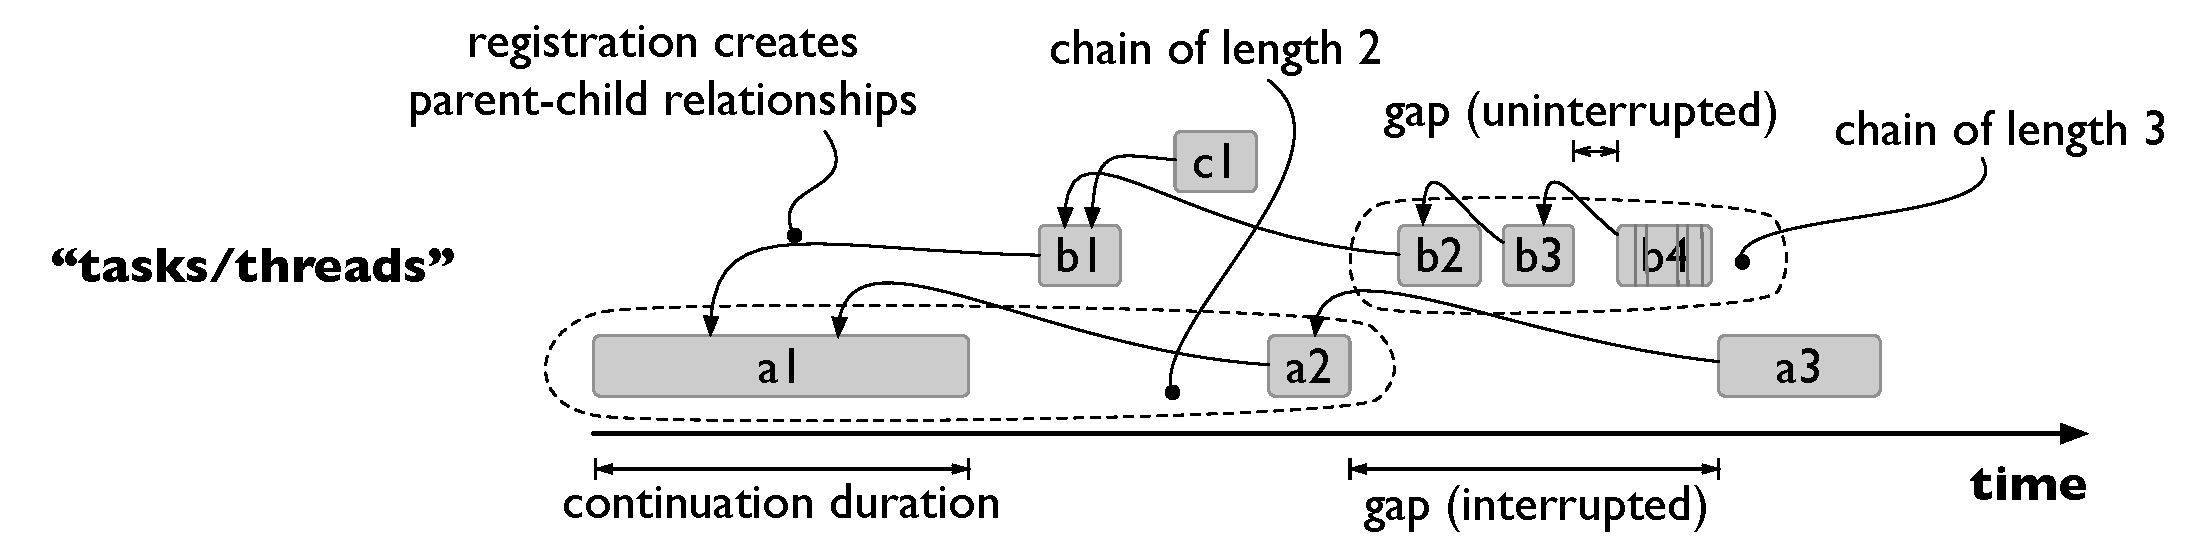
\includegraphics[width=0.9\textwidth]{Figures/continuation_tree}
\caption{The features of JavaScript event execution that our modified Chromium browser measures.
  The gray boxes are continuations.
  The continuations are arranged in rows to suggest that they belong to the same task/thread.
  However, event loop systems do not have this concept, so this is purely an intuitive interpretation.
  For example, a2 and b1 are both children of a1, and there is no way for the system to know what logical task either belongs to.}
\label{fig:continuation_tree}
\end{figure*}

In summary, the contributions of this paper are:
\begin{itemize}
\item A measurement study of multitasking in web applications.
\item An analysis of the conflict between atomic blocks and anonymous multitasking.
\item An exploration of integrating cooperative threading with atomic blocks into an existing multitasking ecosystem.
\item A new call frame allocation strategy for languages with atomic blocks.
\end{itemize}

All code and data described in this paper is available publicly on GitHub [URL removed for blind review].

\section{Multitasking in Web JavaScript}

We begin with a brief (and partial) history of multitasking in JavaScript.
In the beginning, the designers of JavaScript decided that preemptive threads caused an unacceptably high risk of concurrency bugs.
One good entry into the vast literature on the difficulties of diagnosing and fixing multithreading defects is \cite{Lu2008}.
These challenges have long been understood; more than two decades ago Ousterhout wrote a popular critique of threads \cite{Ousterhout1996}.

Early versions of JavaScript supported only event-based concurrency.
The simple picture of the implementation of JavaScript is that there is a single event dispatcher that stores a collection of functions waiting for some enabling condition.
These functions can be registered by primitive APIs, like \texttt{setTimeout}.
In all cases we refer to such registered functions as \emph{continuations}.
We refer to a continuation plus its enabling condition as an \emph{event}.
When an event becomes ready, the dispatcher may execute its continuation whenever it chooses (generally as soon as possible).

Simple event programming has some serious drawbacks.
Management of resources whose lifetime spans multiple events can be quite tricky.
This leads to a style of programming referred to as \emph{stack ripping} \cite{Adya2002}, or more colloquially \emph{callback hell}.
These and more subtle problems are well analyzed and criticized by von Behren et al. in \cite{Behren2003a}.

The increasingly sophisticated multitasking in modern applications and the well-known problems with events and threads have increased the use of alternatives in recent years, the most popular of which are \emph{coroutines} and \emph{async procedures}.
Examples include async/await, which was added to C\#/.Net in 2012; function generators (\texttt{function*}), which were added to JavaScript with ECMAScript 6 (standard published in 2015); even the staid C++ community is considering adding native support for coroutines (currently on the short list for inclusion in the C++20 standard).
Coroutine implementations are not \emph{new}; for example, Modula-2 had coroutines in the 1980s and several ``scripting'' languages (Ruby, Python, Lua) added support in the early aughts.
However, coroutines were not widely used in application programming until relatively recently.

The most recent versions of JavaScript support both coroutines and async functions.
A style of programming that combines async functions and Promise chaining has become popular in JavaScript communities.
This style of programming makes multitasking much more convenient than programming with explicit callbacks.
This evolution in style has made it feasible for more developers to write more highly multitasked applications.

The theme of the measurements in the remainder of this section is: perhaps there are ways in which it is now too easy to write highly asynchronous code.
In particular, the atomicity safety of JavaScript and similar languages has always relied heavily on relatively long-running (in the microscopic computer clock rate sense) uninterruptible functions.
As programmers chop applications up into chains of smaller functions, atomicity problems reemerge as an interesting risk.

\subsection{Measurements}

We modified a version of Chromium to gather data on JavaScript behavior from web applications.
Figure \ref{fig:continuation_tree} illustrates the features of JavaScript execution that our modified browser measures:

\begin{itemize}
\item Continuation duration is the time difference between when the dispatcher passes control to a continuation and when it returns.
\item We measure both the duration and number of microtasks in microtask batches.
  More on microtasks below.
  (The vertical lines in continuation b4 in the Figure are meant to suggest individual microtasks within a batch.)
\item Parent-child relationships are inferred by recording which continuation (the parent) is running when potential children are registered; this relation is referred to as \emph{async-contexts} in \cite{Loring2017}.
  There is actually a more subtle distinction between what that paper refers to as \emph{linking contexts} and \emph{causal contexts} when dealing with Promises.
  We will primarily be analyzing raw callbacks, for which this distinction does not exist
\item A \emph{gap} is the time difference between the start of a continuation and the end of its parent.
  A gap is \emph{interrupted} if \emph{any} other continuation runs between parent and child.
\item Figure \ref{fig:continuation_tree} suggests with the horizontal rows an intuitive notion of tasks, where a registered continuation can either be a logical continuation of its parent's task or a newly spawned concurrent task.
  This concept is sufficiently important that several libraries and tools have related ideas, like Zones in AngularJS, Async Hooks in Node.js and Async Call Stacks in the Chrome Developer Tools.
  Unfortunately, it is not part of standard JavaScript, so in general it is not possible to automatically and precisely infer.
\end{itemize}

% Async Hooks. 2016. https://github.com/nodejs/diagnostics/tree/ master/tracing/AsyncWrap.
% Async Call Stacks. 2014. http://www.html5rocks.com/en/tutorials/developertools/async-call-stack/.
% [26] Zones. 2014. https://github.com/angular/zone.js.

\begin{figure}
    \centering
    \begin{minipage}[t]{0.47\textwidth}
        \centering
        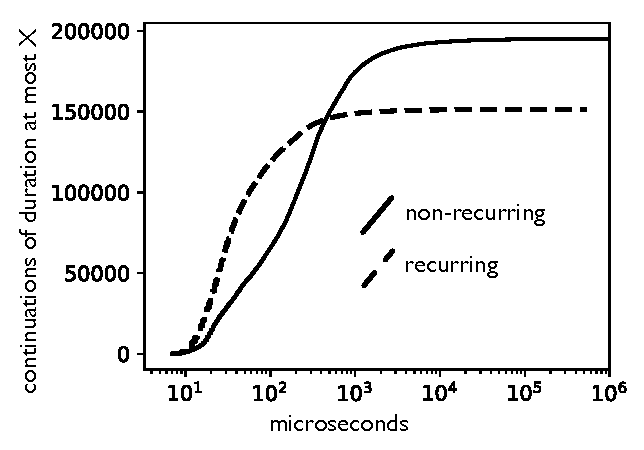
\includegraphics[width=1.0\textwidth]{Graphs/durations_bw}
        \caption{Most continuations are short.
  Many are very short.}
        \label{fig:graph_duration}
    \end{minipage}\hfill
    \begin{minipage}[t]{0.47\textwidth}
        \centering
        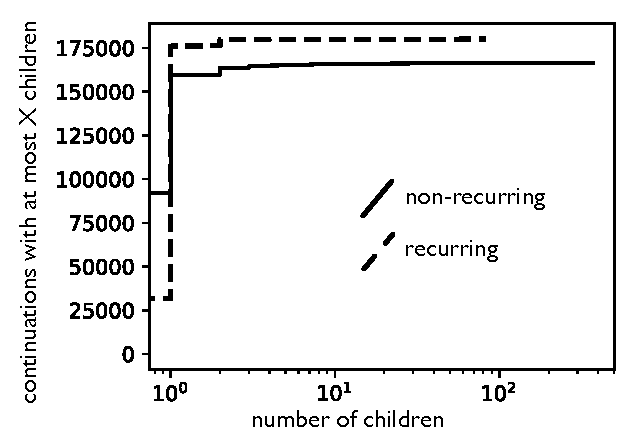
\includegraphics[width=1.0\textwidth]{Graphs/branching_bw}
        \caption{Most continuations have one child.
A few have many, many children.}
        \label{fig:graph_branching}
    \end{minipage}
\end{figure}

\subsubsection{Duration}

Our first observation from Figure \ref{fig:graph_duration} is that most continuations are quite short.
A large majority take less than one millisecond, and many are much shorter.
(This figure combines the data for both microtask batches and normal tasks.)

The shortness of most continuations is \emph{not} direct evidence of atomicity problems.
It is a necessary condition, though; if most continuations were long, we would expect it to be less common for a programmer to ``miss'' a gap between them.
Also, it is interesting to see that JavaScript programmers seem to overwhelmingly abide by the norm that all function executions should complete quickly, in order to keep applications responsive.
This observation will be important when we discuss API design later.

The difference between the solid and dashed lines in Figure \ref{fig:graph_duration} highlights the importance of recurring events.
In JavaScript, certain APIs, like \texttt{setInterval} and \texttt{XMLHttpRequest} register continuations that the event dispatcher can call multiple times.
As you can see, these recurring continuations account for a majority of the shortest.
(A majority of those are accounted for by status updates on downloading files.)
However, even among the non-recurring continuations, there are still quite a few towards the short end of the distribution.
In several of the measurements and analyses below we \emph{filter out the recurring events}, because they are less relevant to our focus on chains of continuations that could be mistaken for being atomic.

\subsubsection{Branching and Concurrency}

Next, notice in Figure \ref{fig:graph_branching} that most continuations have \emph{at most} one child.
Among recurring continuations there are more with one child; among non-recurring continuations there are more with zero.
The fact that there are many single-child continuations suggests that JavaScript programmers are breaking linear sequences of logic up into multiple continuations.
Presumably they are doing this either intentionally to improve responsiveness, or because of libraries that only offer an async interface.
Otherwise, why not combine these continuations into a single one?

Though most continuations have few children, a few continuations have many.
This can be seen in the long tail in Figure \ref{fig:graph_branching}.
(There are at least a few continuations with hundreds of children!)
A consequence of this branching is that the continuation trees we studied exhibit quite a lot of concurrency.
For each continuation we define its degree of concurrency to be the number of continuations that \emph{will} run \emph{after} it, but were registered before it started.
In other words, how many parent-child edges are ``live'' across each continuation?

Figure \ref{fig:graph_concurrency} shows the results of our concurrency measurements.
Notice that most continuations are concurrent with at least 10 edges, and a substantial minority are concurrent with at least 100.
Again, the high degree of concurrency is \emph{not} direct evidence of atomicity problems, but it is another precondition.
If most continuations had a low degree of concurrency there would be little opportunity for a conflicting task to create an atomicity violation.

\begin{figure}
    \centering
    \begin{minipage}[t]{0.47\textwidth}
        \centering
        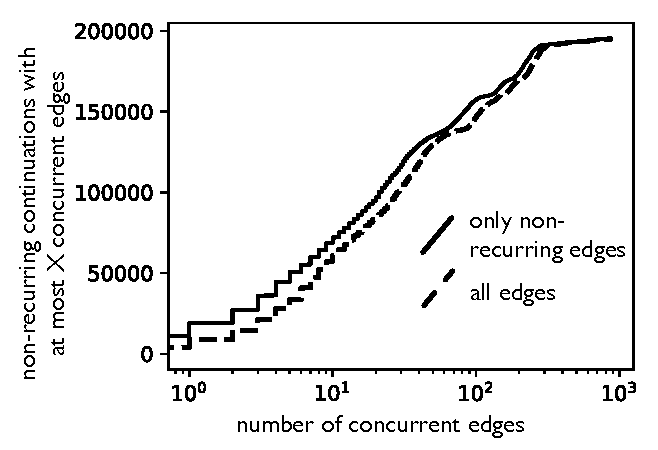
\includegraphics[width=1.0\textwidth]{Graphs/concurrency_bw}
        \caption{Most continuations are concurrent with several parent-child edges.
        In this graph we only include non-recurring continuations.}
        \label{fig:graph_concurrency}
    \end{minipage}\hfill
    \begin{minipage}[t]{0.47\textwidth}
        \centering
        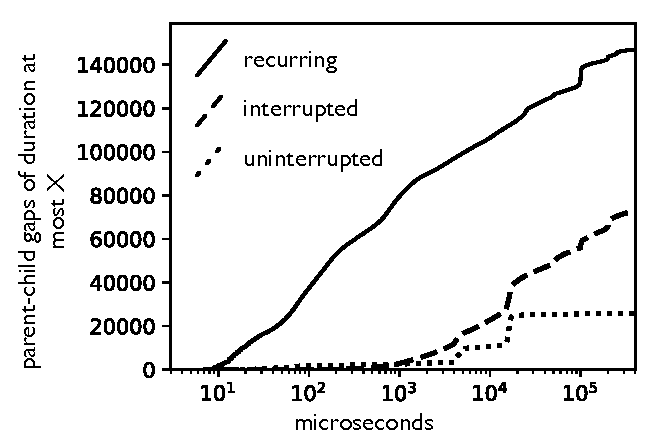
\includegraphics[width=1.0\textwidth]{Graphs/gaps_bw}
        \caption{Most gaps are of reasonable length, but a nontrivial percentage are quite short (under one millisecond, or even 100 microseconds).
  This graph is truncated at half a second, because we are not interested in long gaps.
  There is only a small number of longer gaps.}
        \label{fig:graph_gaps}
    \end{minipage}
\end{figure}

\subsubsection{Gaps and Chains}

The last basic measurements of continuation trees that we consider are the lengths of parent-child gaps and short chains.
Figure \ref{fig:graph_gaps} shows that many gaps are quite short.
The majority of the shortest gaps are between recurring events, which are less interesting to us.
However, there are still quite a few gaps between non-recurring events that are below 10 milliseconds.

A particularly interesting feature to notice is that there are thousands of uninterrupted gaps in the 100s of microseconds range, but far fewer interrupted gaps.
This means that interruption of gaps of that size is possible, but rare.

Figure \ref{fig:graph_chains} shows the duration of continuation chains of length 2, 3 and 4 (that is, the time difference between the beginning of first continuation in the chain and the end of the last).
For this graph we filtered out all chains with recurring continuations.
This data is not surprising based on the continuation duration and gap data and presented above.
We see that while many chains are of a fairly reasonable duration (say, dozens to hundreds of milliseconds), there is a non-trivial fraction under 10 milliseconds, and even some under 1 millisecond.

Yet again, short gaps and short duration chains are \emph{not} direct evidence of atomicity problems.
However, it is easy to imagine a rigorous testing regime that never observed an execution where one of these short gaps was interrupted.

\begin{figure}
    \centering
    \begin{minipage}[t]{0.47\textwidth}
        \centering
        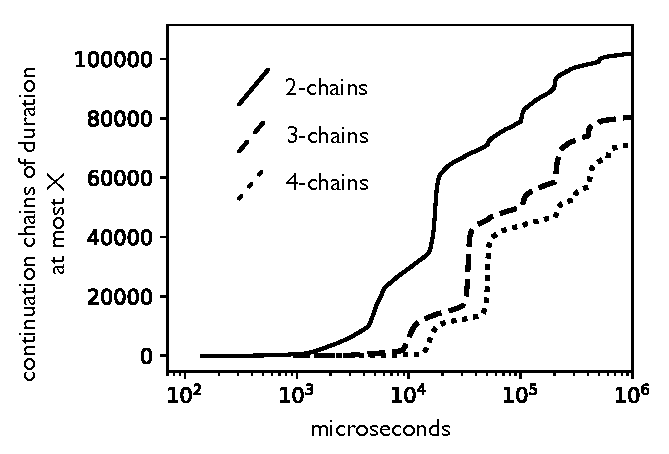
\includegraphics[width=1.0\textwidth]{Graphs/chains_bw}
        \caption{XXX chains.}
        \label{fig:graph_chains}
    \end{minipage}\hfill
    \begin{minipage}[t]{0.47\textwidth}
        \centering
        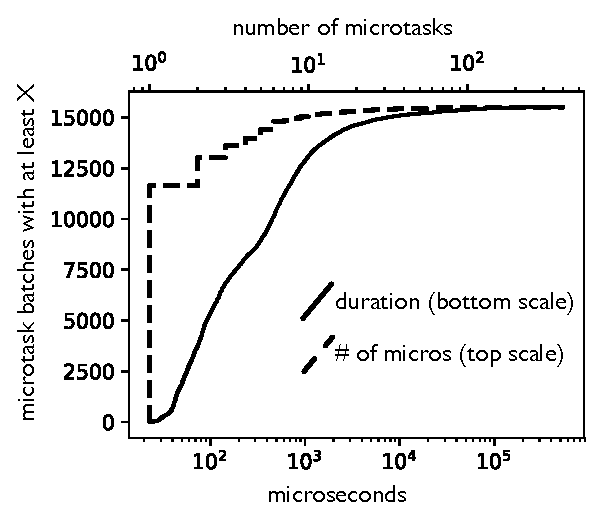
\includegraphics[width=1.0\textwidth]{micros_graph_bw}
        \caption{Most microtask batches are short, but a nontrivial number are long enough to possibly exceed the time and/or microtask count limits of some reasonable implementations.}
        \label{fig:graph_microtasks}
    \end{minipage}
\end{figure}

\subsubsection{Microtasks}

In this subsection, we look at microtasks, which are tangential to the main plot of this paper, but still somewhat interesting.
Microtasks are a special subset of events in JavaScript; the most common source of microtasks is Promise resolution.
Unlike regular events, as soon as at least one microtask is registered, the interpreter switches to running microtasks.
During the execution of a microtask, more microtasks can be registered, and the interpreter will not run another continuation from the normal event dispatcher until the microtask queue is empty.

Figure \ref{fig:graph_microtasks} shows information about the durations and microtask counts of microtask batches.
Most batches are fairly short/small by both metrics, which is good from a concurrency bug perspective.
However, a nontrivial minority of microtask batches get into the 10s and even 100s of milliseconds and/or dozens or hundred of microtasks.
At that size, these microtask batches start to be potential responsiveness problems.
When batches of microtasks get too long, programmers may make ad hoc decisions about where to break them up, thus potentially creating more opportunities for atomicity problems.

\subsection{Instrumentation, and Data Source Details}

TODO

\subsection{Is This Actually a Problem?}

In this paper we do not present any specific atomicity violations, only evidence that risky patterns are common.
This leads us to a couple interesting questions:
How confident can we be that the patterns we study are associated with real atomicity defects, and are thus worth doing something about?
If these patterns are a valid concern (of any magnitude), what explains their existence in the most widely used web applications?
We will address the second question first.

\subsubsection{An Explanation for the Rise of Short Chains}

There is always a dilemma in cooperative concurrency models associated with the durations of whatever the atomic chunks are in that model.
The longer the chunks are, the higher the risk of unresponsiveness or at least appearing jittery and potentially missing I/O deadlines.
The shorter the chunks are, the higher the risk of splitting some logic that should be atomic into multiple chunks.

This dilemma is particularly acute for library authors, because they bear the responsibility to make their code work well in multiple specific contexts; quite often many of the contexts are unknown to the library authors.
To be more concrete, when library authors design APIs, they face the choice between making a call atomic or async in some way (callback, Promise, async method, whatever).
In some cases this choice is easy.
If the function will always complete in a small amount of time, then it should be atomic.
If the function will usually take a long time, then it should be async.

Unfortunately, many functions fall in the awkward middle territory, where in some contexts they complete quickly and not in others.
For these functions, async is in some sense the easier choice, because long-running atomic calls create immediately obvious responsiveness problems that cannot be easily worked around by applications.
On the other hand, atomicity problems are not as obvious and in principle can be worked around by application-level synchronization.

A similar line of reasoning led the developer's of Microsoft Windows' core Windows Runtime (WinRT) library to replace many atomic procedures with asynchronous ones in Windows 8.
In a post on the Microsoft Developer Blog \cite{Windows8Team2012}, the team explains that they did this for procedures that ``could likely take longer than 50 milliseconds to execute''.

In some recently defined JavaScript APIs, even some functions that will execute quickly in most reasonable contexts have an async interface.
As one example among many, the PBKDF2 key derivation function in the cryptography API returns a Promise.
PBKDF2 is a function that takes a number of iterations as a parameter.
On a modern computer the PBKDF2 function takes in the rough neighborhood of one microsecond per iteration.
So the iteration parameter must be set very high for this function to represent a responsiveness problem.
In contexts where the iteration count is lower, the caller would almost certainly prefer an atomic interface.

Consider a more extreme example: sending a network request.
Sending a message over a wide area network will inevitably be slow, and network operations are generally defined to be asynchronous to accommodate this.
However, in a microservices software architecture, applications use network protocols to communicate with other processes that might be running on the same computer.
Depending on the details of a specific request to a peer process, it may actually be fast enough that the requester would prefer to block while waiting for the response.

These examples illustrate what we claim is a general trend towards giving library functions an async interface.
We further claim that the data presented in the last section can be seen as a consequence of this trend.

SPAs, end-to-end encryption

\subsubsection{The Atomicity Violation Struggle is Real}

There has been a great deal of research on atomicity violations in general (for example, \cite{Lu2008}).
More directly relevant to this paper, several researchers have worked on detecting and classifying concurrency bugs in event-driven web and mobile applications: \cite{Petrov2012, Hsiao2014, Mutlu2015, Zhang2017}.
These papers focus on ``races'', which are related to atomicity violations, but easier to study in the sense that races can be defined without dealing with application logic. XXX

% Petrov2012  Race Detection for Web Applications
% Hsiao2014  Race Detection for Event-driven Mobile Applications
% Mutlu2015  Detecting JavaScript Races That Matter
% Zhang2017  RClassify: Classifying Race Conditions in Web Applications via Deterministic Replay
% XXX Shin Hong, Yongbae Park, and Moonzoo Kim. Detecting concurrency errors in client-side java script web applications. In IEEE International Conference on Software Testing, Verification and Validation, pages 61– 70, 2014.

Another kind of evidence is analysis of concurrency bugs in JavaScript applications based on real bug databases: \cite{Davis2017, Hong2014, Wang2017}.
The authors of \cite{Davis2017} reported that 69\% of the 16 concurrency bugs they studied involved an atomicity violation, while the authors of \cite{Wang2017} reported 65\% of 57 bugs.
The latter paper goes on to report that of the atomicity violation bugs, 27\% were fixed by adding synchronization or switching to an atomic API.
These papers specifically looked at applications based on Node.js, which is somewhat different from browser JavaScript.
However, with the rising popularity of tools like Webpack, Browserify and Gulp, libraries from the expansive NPM ecosystem are being used increasingly in code written for browsers.
This means that the differences between browser JavaScript and Node.js JavaScript are shrinking.
Also while Node.js has traditionally been used to develop backend servers, it is increasingly being used directly in client applications via tools like Electron, Cordova and Ionic.

% Davis2017 11/16 atomicity violations
% Wang2017  65% atomicity violations --> 27% fixed by adding synchronization or switching to an atomic API

\subsubsection{Potential Solutions}

The remainder of this paper explores atomic blocks as a mitigation strategy for atomicity problems.
However, we do want to acknowledge that there are other strategies that programmers are surely already using to some extent.

One strategy is to use a ``functional'' style of programming, with immutable data structures and application-level atomic transactions.
If this strategy is used consistently, then it is unimportant how small the atomic chunks are; the correctness of the program depends very little on fine-grained scheduling.

Even if a project is written in the more common imperative style with fine-grained actions with observable effects, careful software engineering can still protect against atomicity violations.
For example, programmers could use an adversarial scheduler during testing to flush out concurrency bugs.

While the authors of this paper have no quibbles with either of these strategies, we observe that quite a few applications are written with a modest level of software engineering care.
It would be nice if there was a relatively simple tool (like an atomic block) that could help avoid at least some subset of concurrency issues.
Also one note of caution to keep in mind is that some techniques are appropriate for maintaining atomicity within the bounds of a single process, but are less relevant when I/O is involved.

\section{The Tension Between Anonymous Multitasking and Atomic}

\begin{figure}
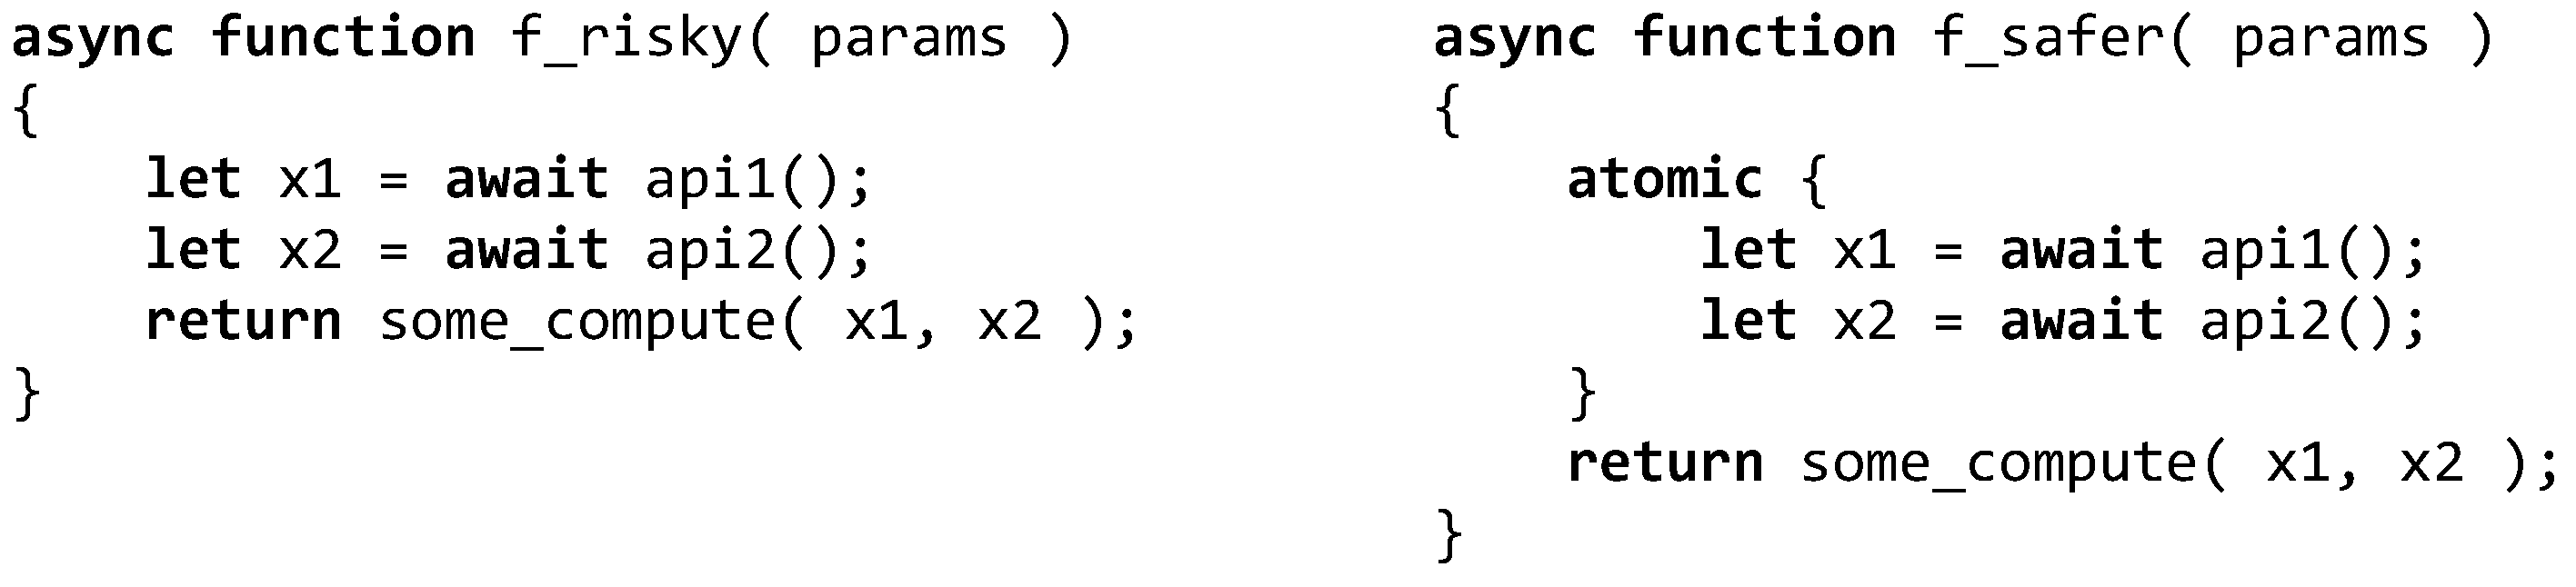
\includegraphics[width=0.3\textwidth,left]{Code/async_atomic_js}
\caption{A simple example of code that could lead to the risky gaps, and a version with an atomic block to eliminate the risk of an atomicity violation.}
\label{fig:async_atomic_js}
\end{figure}

As discussed in the previous section, there are multiple viable strategies for mitigating the risk of atomicity violations created by short-duration chains of continuations.
In this section we explore one of those strategies: adding an atomic block to languages like JavaScript that use event loops, coroutines or similar anonymous multitasking frameworks.
Figure \ref{fig:async_atomic_js} shows a very simple example of how atomicity violations can arise, and our proposed solution.
Previous research has shown that atomic blocks can be an effective concurrency control mechanism in the multithreading context (for example, \cite{Pankratius2011, Pankratius2014}).
Most importantly for this project, atomic blocks are simpler to use than some alternatives (e.g. explicit mutex locks), and therefore are useful to developers of a wider skill range\footnotemark{}.

\footnotetext{Despite considerable attention from the research community, atomic blocks have not become a common feature in the context of multithreading.
We believe this is primarily due to the substantial implementation challenges and tricky semantic issues with how code in an atomic block should interact with concurrent code that is not in an atomic block.
These issues are not relevant in a cooperative context.}

In this section we show that the combination of anonymous multitasking (e.g. with event loops or coroutines) and atomic blocks is problematic.
We then explore adding a flavor of cooperative threads with atomic blocks to JavaScript.

\subsection{A Definition of Atomic with Event Loops}

One way atomic could be defined in event systems is as follows:

\cite{Loring2017} Semantics of Asynchronous JavaScript

\begin{enumerate}
\item When some code enters an atomic block, all pending events are removed from the dispatcher and pushed collectively onto a stack of pending events.
\item The code of the atomic block runs as usual, possibly registering new events.
\item When the code reaches the end of the atomic block it pauses to allow events from the dispatcher to run (i.e. the events registered by the atomic block itself).
\item Events are executed as usual (with continuations potentially registering new events).
\item Once the event dispatcher is empty, the code that was waiting at the end of the atomic block can continue; simultaneously the events that were pushed in step 1 are restored to the dispatcher.
\end{enumerate}

Notice that this definition is reasonable for nested atomic blocks.
In cases where the body of an atomic block consists of a linear chain of continuations, this definition would produce exactly the expected effect: the whole chain would run before any concurrent events are processed.
It is when when there is branching within the atomic block that the desired semantics get less clear.
Because it is not possible to distinguish between logically continuing the current task and spawning a new one, this definition effectively assumes that all continuations are part of their parent's task, and assumes they should all be contained within the atomic block.

\subsection{Background on Nested Atomics and Spawns}

In this subsection we give a brief review of research on atomic blocks in the context of multithreading and transactional memory.
We will relate this back to event loop systems below.
The tricky semantic issue is how to define thread spawns nested within atomic blocks (and potential further nesting of both).
One good treatment of the formal semantics of this issue is \cite{Moore2008}.
Some of the possibilities that have been explored are:
\begin{itemize}
\item Spawning a thread within an atomic block is a dynamic error.
\item Spawning a thread within an atomic block is a static error.
\item Threads spawned within an atomic block are delayed until just after the block has completed. (\emph{delay-spawn})
\item Threads spawned within an atomic block are allowed to run concurrently, and the block is not complete until such threads are finished. (\emph{spawn-contained})
\item Threads spawned within an atomic block are allowed to run concurrently, and are completely disconnected from the block.
\end{itemize}

Unfortunately, it seems there is no simple definition that works well in all cases.

Disallowing spawning inside of atomic blocks (either statically or dynamically) is tempting, since it somehow feels like spawning new tasks is not in the spirit of ``atomic''.
However, such rules are hard to defend on principle, because there are perfectly reasonable programs that have spawns inside atomic blocks.
Furthermore, as we will see in the empirical analysis below, programs that seem to have this shape are fairly common.

The \emph{delay-spawn} strategy causes deadlock for code that spawns a thread then waits for it, while still in the atomic block.

The \emph{spawn-contained} strategy causes starvation for code that spawns long-running tasks, because according to this strategy the atomic block is not finished until all tasks are finished.

%% A quick example of when the \emph{spawn-contained} policy is problematic:
%% Consider a function that performs a few quick database queries and then sends a potentially slow network request based on the results of the queries.
%% A caller may want to enforce atomicity among the database queries, but wrapping a call to this function in atomic would cause the application to become unresponsive until the network request completed.

\subsection{Do Programs Actually Do this Weird Stuff?}

\begin{table}
  \centering
  \begin{tabular}{|r|r|r|r|r|r|r|}
    \hline
    Limit (ms) &  Total & Linear & Multi L & Multi S & Contain L & Contain S \\
    \hline
    1          &    837 &   66\% &    17\% &   0.7\% &      18\% &     0.2\% \\
    \hline
    10         & 17,885 &   80\% &   4.4\% &   2.1\% &      15\% &     1.3\% \\
    \hline
    100        & 46,515 &   87\% &   3.9\% &   2.3\% &     8.3\% &     1.5\% \\
    \hline
  \end{tabular}
  \caption{XXX subtrees}
  \label{table:subtrees}
\end{table}

Before considering approaches to handing nested atomics and spawning, it is useful to consider whether these patterns seem to actually occur in applications.
If it seems that spawning in atomic blocks is rare, then simple solutions (like making it an error) might be viable.

We analyzed the continuation trees we collected for evidence of spawning within atomic blocks in the following sense.
Obviously JavaScript lacks both atomic and explicit spawning and atomic blocks, so out analysis is inevitably guessing to some extent.
We define potentially atomic subtrees in the continuation trees to be those that satisfy the following conditions:

\begin{itemize}
\item \emph{Nontrivial}. At least two continuations.
\item \emph{Connected}. Not forests.
\item \emph{Time limited}. The duration from the beginning of the first continuation to the end of the last can be at most some specified limit.
\item \emph{Maximal}. Proper subtrees of trees that satisfy these conditions do not count.
\item \emph{No Recurring}. Recurring edges are ignored, except for a special case described below.
\end{itemize}

We examined the shape of the potentially atomic subtrees, and found the following shapes.
For some shapes we defined variants of the criteria that we call ``looser'' or ``stricter''.

\begin{itemize}
\item \emph{Linear}. All continuations have at most one child.
  For this one we considered recurring edges as well -- ``truly linear''
\item \emph{Multiple long-lived branches}. Looser version: At least two children outside the subtree (can have the same parent).
Stricter version: At least two children outside the subtree with different parents.
\item \emph{Contained branch}. Looser version: At least one continuation with no children, and at least one continuation with at least one child outside the subtree.
  Stricter version: Same as the loose version, with the additional constraint that there be at least one continuation in the subtree after the one with no children.
\end{itemize}

The quantitative results are in Table \ref{table:subtrees}.
The first thing to observe is that most of the subtrees are linear, but not by an overwhelming margin.
A definition of atomic blocks that handled branching poorly would likely create substantial problems for programmers.


An issue with event-based concurrency is that there is no explicit notion of a task or thread that defines the identity of specific chains of continuations.
In other words, when a continuation is registered, the system cannot be sure whether it is logically continuing the execution of its parent or spawning a concurrent task.

The simple strategy sketched above effectively assumes that all continuations spawned during an atomic block belong to their parent's task.
Therefore, the dynamic scope of the atomic block must include all children, grandchildren, etc until all newly registered continuations have completed.
This corresponds closely to the \emph{spawn-contained} policy.


We conclude that adding an atomic block directly to an event system is possible, but problematic.
We believe that a much better option is to introduce an explicit notion of tasks/threads, which is what the next section explores.

We briefly note that there are other options for defining an atomic block in an event system.
For example, the system could assume that the last child registered by a continuation is part of its parent's task and any other children are concurrent tasks.
We do not investigate these options further, because they seem too ad hoc.

\subsection{Risks of Unresponsiveness}

Variability in duration of different dynamic instances of the same static atomic block ...

\section{Cooperative Threads and Atomic Blocks for JavaScript}

Doppio ??? \cite{Vilk2014}

In this section we discuss the first of our two implementations of cooperative threading with atomic blocks.
Atomic blocks have been at least experimented with in the context of preemptive multithreading in several other languages, for example: Haskell \cite{Harris2005}, OCaml \cite{Ringenburg2005}, Java \cite{Herlihy2006}, C/C++ \cite{Ni2008}.
We do not claim any novelty with respect to the basic questions of what atomic blocks should mean.
In fact, it should be much easier to implement atomic blocks in the cooperative context.
The interesting points we explored were how easily our library could be integrated with popular coding patterns and legacy code.

In this section we discuss a library implementation of explicit tasks in JavaScript, built on top of async functions.
Async functions were standardized in ECMAScript 2017.
It is also possible to define async functions as a library, built on top of JavaScript's function generators (\texttt{function*}) and Promises.
In fact, there are many examples of such libraries added to JavaScript frameworks for convenience.

\begin{figure}
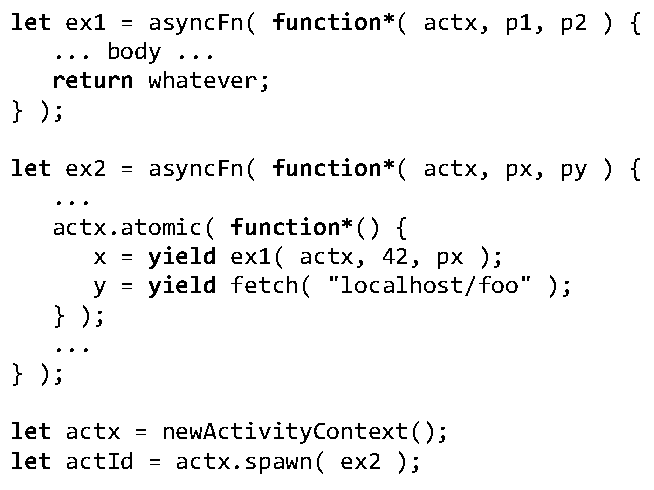
\includegraphics[scale=0.65]{Code/trivial_js}
\caption{A sketch of how the JavaScript library implementation of activities is used.
The syntactic clutter is fairly high because we are using JavaScript function generators (\texttt{function*}) to simulate regular functions in an activities framework.}
\label{fig:trivial_js}
\end{figure}

Our library has two essential functions: spawn and atomic.
Spawn takes an async function as a parameter and returns a handle to a concurrent task.
In our library we call these concurrent tasks \emph{activities}.
Atomic takes a function generator as a parameter and ensures that it runs atomically (i.e., it is not interrupted by an concurrent activities).

Figure \ref{fig:trivial_js} gives a tiny example of what our library actually looks like.
Notice that each asynchronous function needs an additional context parameter so that it can know what activity it belongs to.
If this were implemented natively in a language, this parameter would be unnecessary.

Without atomic and spawn nesting, the implementation of this library would be relatively simple.
There would be a single global variable that contained either null or the identity of the activity in atomic mode.
Each async function would need to know the identity of the activity it belongs to, and would check the global variable before resuming.
If the variable contains the identity of some other activity, the async function would need to wait.
Upon exiting an atomic block, any waiting async functions would be released.

Because we want it to be legal to spawn inside of an atomic block, the single global variable indicating \emph{the} activity that is in atomic mode is no longer sufficient.
Instead we need a stack of sets of activity identifiers, which is initially empty.
When an activity enters atomic mode, it pushes a singleton set on the stack with its own identifier.
When an async function attempts to resume it now needs to check whether the stack is empty (i.e. no activity is in atomic mode) or if it is in the set on top of the stack; if neither is the case, then it must wait.

As mentioned previously, there are several reasonable strategies for handling spawns inside atomic.
By default, activities spawned while the program is in atomic mode will be put on hold until the program has exited atomic mode.
This strategy is the default because it is relatively simple, and as long as the atomic block executes relatively quickly (which is how the feature is supposed to be used), the newly spawned activities will experience relatively little delay.
Unlike the multithreading and transactional memory context, where there might be a performance benefit to letting multiple threads simultaneously execute in atomic mode, we are dealing with single-threaded multitasking here.

The only situation in which the \emph{delay-spawn} strategy is problematic is when the code executing the atomic block waits (directly or indirectly) for the newly spawned activity to do something before leaving the atomic block.
In this situation, forcing the new activity to wait could cause the program to deadlock.
For this reason, the spawn function accepts an optional parameter to override the default nesting strategy.
Newly spawned activities can be spawned with the \emph{spawn-contained} strategy.
This allows the newly spawned activity to run, and forces the program to wait at the end of the atomic block for any such activities to complete.

We briefly note an efficiency opportunity that atomic blocks create.
In addition to being an atomicity hazard, chains of short continuations create event dispatcher overhead.
In a version of JavaScript with an atomic block, it would be possible for a just-in-time compiler to fuse continuations run atomically into a single function, reducing this overhead.

The \emph{activities} design we ended up with is essentially cooperative threads plus automatic yield insertion around async functions and atomic blocks.
In this paper we do not present a formal semantics for activities.
Rather, we refer to existing work on the semantics of cooperative threads \cite{Abadi2009} and atomic blocks \cite{Moore2008}.
The semantics of activities are a combination of these two ideas.

\subsection{Integration with Legacy Code}

Our activities library integrates relatively cleanly with legacy JavaScript code.
Any JavaScript Promise can be yielded, just as one would with regular async function implementations.
One small awkwardness is that our library cannot prevent continuations registered by legacy code from running whenever the event dispatcher chooses.
So if one activity is in an atomic mode, a continuation previously registered by legacy code run in another activity may still run.

\subsection{Building an App with Activities}

Our experience with the JavaScript Activities library consists primarily of building a simple single-page web app that lets users share information.
It makes heavy use of the cryptography API to implement an end-to-end encryption protocol.
We wrapped the Promise-returning API functions with simple \texttt{asyncFn}s.
There is a high density of calls to such functions in the code.

We make a couple observations about this experience.
First, compared to an earlier version of this app that used explicit callbacks, the direct style is dramatically easier to read and reason about.
Of course, using async functions would also give this benefit.

More than half of the calls we expect to be short-lived.
These we can execute in atomic mode to ensure that there are no atomicity violations around them.
Using standard async functions, it would not be possible to do that.

\section{An Atomic Block for C (Design)}

In the previous section we did not discuss the efficiency of the JavaScript implementation of activities in any detail.
However, we are interested in whether activities can be implemented in a highly efficient way, so we added them to a dialect of C that we call \charcoal{}.
In this section, we discuss the design of \charcoal{}.
In the next section we discuss the implementation of \charcoal{}.

Like the JavaScript version, the primary additions are spawn and atomic primitives.
We also needed to add a yield primitive, since this does not exist in plain C.
The main differences with the JavaScript version are related to the manual memory management of C.

To illustrate our design, we use an example stolen from \cite{Krohn2007}; a plain C version is in Figure \ref{fig:charcoal_multidns_seq}.
This example performs \texttt{N} DNS lookups using the standard \texttt{getaddrinfo} procedure.

The \charcoal{} version performs in Figure \ref{fig:charcoal_multidns_sem} performs these lookups concurrently.
It has a parameter (\texttt{max\_conc}) to limit the number of DNS requests that will be sent concurrently to avoid flooding the network with too many requests.

In \charcoal{} we add some syntactic convenience to the plain spawn to get the \emph{activate} statement, an example of which is on line 10 of the example.
The body of the activate statement runs concurrently (but \emph{not} in parallel) with the statement's continuation.
Only one activity can be running at a time and the system can only context switch between activities on a yield.

\begin{figure}
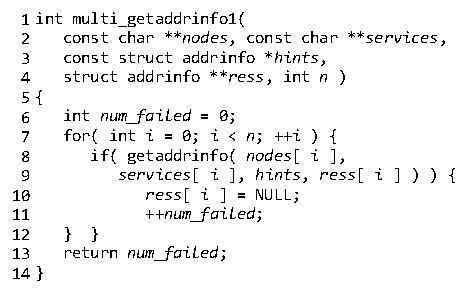
\includegraphics{Code/multi_getaddrinfo_seq}
\caption{This is a plain C version of the DNS fetcher running example.
  This version is entirely \emph{sequential}.}
\label{fig:charcoal_multidns_seq}
\end{figure}

Each \charcoal{} program has a scheduler that chooses when a yield should lead to a context switch, and which activity to switch to.
The current \charcoal{} implementation uses a simple FIFO scheduler; clearly this is something that could be looked at for further refinement in terms of performance, fairness guarantees and/or greater application control.

The activate statement takes as a parameter a pointer to application-allocated memory for storing metadata about the new activity.
In the example, the memory for storing activity information is allocated locally.
Because of this the example procedure must wait for all the activities it spawns to finish.
(Returning before they finish could cause the program to access deallocated memory).
It would be possible to change the interface so that the caller passes in the backing memory, or to use dynamic allocation and leave the deallocation to the caller.
In either of these cases, the procedure could return while the activities were still fetching DNS information, allowing the application to go on with other work.

\subsection{Shared Variables}

The parentheses after the \texttt{activate} keyword are for controlling whether local variables are accessed by-value or by-reference.
The default is by-reference, which is how most of the variables are used in this example.
This means that all the activities read and write a shared instance of that variable.
The exception is \texttt{i} which is used as a name of sorts in the \texttt{printf} call.
Each activity gets its own copy of \texttt{i}, whose initial value is whatever the variable's value was at activity creation time.
If there were a modification to \texttt{i} inside \texttt{activate}, each activity would be modifying its own copy.

\subsection{Yield Insertion}

One of the two primary features that distinguish activities from conventional cooperative threads is that there is a translation step that automatically inserts yield statements before and after every procedure call.
This rule helps ensure responsiveness by default.

There are two ways a program can still become unresponsive.
The first is by wrapping a long-running part of the program in atomic.
The second is long-running loops with no calls (or explicit yields) in their body.
Both of these should be considered concurrency bugs to be managed with the usual software reliability tools (testing, code review, verification, etc).

\begin{figure}
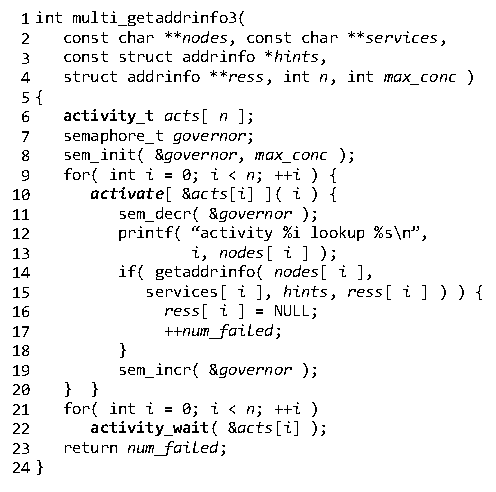
\includegraphics{Code/multi_getaddrinfo_sem}
\caption{This version of the DNS fetcher limits the number of concurrent requests to \texttt{max\_conc}.}
\label{fig:charcoal_multidns_sem}
\end{figure}

In the example code above, the system will automatically insert four yields: one each before and after the two calls.
Without further information, it should be assumed that the called functions themselves have more yields in their implementations.

Automatic yield insertion makes activities more like preemptive threads than conventional cooperative threads.
However, activities are still more resistant to concurrency bugs than threads by default, because the granularity of scheduling is coarser.
Between calls and explicit yield invocations, code is guaranteed to execute atomically.
For example, classic data races are impossible with activities.

\subsection{Atomic}
\label{sec:atomic}

Any statement, expression or procedure declaration in \charcoal{} can be ``wrapped'' with atomic.
In the dynamic scope of a atomic block, the current activity cannot be interrupted.
In other words, any yields that would have happened are overridden/suppressed by atomic.
This is a simple and powerful tool for enforcing atomicity.
Most locking in current multithreading practice can be either removed entirely, thanks to the coarser scheduling granularity, or directly replaced by the simpler and safer atomic.

In the example, the compiler will insert yields before and after the calls to \texttt{printf} and \texttt{getaddrinfo}.
If the programmer wanted to suppress some of these yields, they could use \atomic{}.
For example, it would be reasonable to wrap the \texttt{printf} call in \atomic{}, since it will complete quickly (relative to \texttt{getaddrinfo}), and there is little to be gained by switching to another task at that point.
Wrapping the \texttt{getaddrinfo} call in atomic would be a performance bug, because that would force the DNS lookups to be executed sequentially.

As with the JavaScript implementation, spawns inside atomics are a challenge.
Our solution here is the same: a stack of sets of activities running inside the atomic.
There is an additional challenge here with stack management that we address in the next section.

\subsection{System Calls}

System calls present a challenge, because clearly a language cannot force the operating system to yield in the middle of kernel code execution.
To implement activities correctly, the system must ensure that system calls are performed asynchronously.
That is, during a system call the system may switch to another activity.
If a system call completes while some other activity is running, the calling activity must wait for a yield before it can resume execution.
There are more details on this in the implementation section.
Legacy code can call blocking system calls, which will cause the whole application to block.

\section{An Atomic Block for C (Implementation)}

There are a few interesting features of our implementation of activities in the context of \charcoal{}, which we describe in this section: the allocation of call frames, the implementation the yield primitive, and compiling a version of each procedure for yielding and atomic mode.

\subsection{Call Frame Allocation}

One of the implementation issues for any thread-like abstraction is the allocation of procedure call frames.
The first few sections below briefly review existing strategies for frame allocation.
Then we describe a new approach that we call \emph{hot stacking}.

\subsubsection{Contiguous Allocation}

A common and simple strategy is to pre-allocate moderately large per-thread blocks of memory for that thread's frames.
Individual frames are allocated contiguously within this area.
This strategy is leads to the fastest calling and returning.
However, it can be quite memory inefficient, and if there is a mistake that leads to a thread's stack area being too small a variety of nasty failures can happen.

\subsubsection{Individual Heap Allocation}

At the other extreme of the time/memory efficiency spectrum, systems can individually allocate each frame, linking them together with pointers.
This avoids the memory concerns associated with contiguous allocation.
However, heap allocation of frames comes at a time cost for calls and returns.

Simple implementations of heap allocation can be more than an order of magnitude slower than contiguous allocation.
More sophisticated implementations can be substantially more efficient (e.g. \cite{Shao2000}).
However, even the most efficient implementations that we are aware of are still slower than contiguous allocation for call-heavy code.

\subsubsection{Split/Segmented Stacks}

Some languages have experimented with a hybrid strategy called \emph{split}, \emph{segmented}, or \emph{linked} stacks.
The idea is that stack space is allocated in small segments or chunks.
In the common case, frames are allocated contiguously within the top segment.
When a thread reaches the end of its segment it allocates a new one and links them together with pointers.
This idea has been appealing to several language implementers; as fairly recent examples, early implementations of Rust and Go both used it.
Unfortunately it has unpleasant \emph{uncommon} case behavior called \emph{stack thrashing} or the \emph{hot split} problem.
When there are frequent calls/returns right at the boundary of a segment, the overhead can be quite high.
The implementers of Rust \cite{Anderson2013} and Go (search ``contiguous stacks in go'') both abandoned split stacks in later versions.

% Also \cite{Middha2008}

\subsubsection{Growable Contiguous Stacks}

Since version 1.3, the Go language has used a novel stack allocation strategy, where each thread's stack memory is initially small and is resized on-demand.
This is only possible because the Go language implementation knows about all pointers to stack memory and can update them if necessary (i.e., if it is necessary to relocate the whole stack).
Clearly this would not work for languages like C and C++ that allow application code to use raw pointers.
Similarly to the hot split problem, this strategy suffers from unpredictable pauses when the stack has to be relocated.

\subsubsection{Hot Stacking}

The call frame allocation strategy introduced in this paper is a hybrid of contiguous and individual heap allocation.
The key observation is that the speed of individual allocation is only important for short-lived calls.
For long-lived calls, the overhead of the call and return operations can be amortized over the long running time of the call.
So the main idea of hot stacking is that long-lived frames are individually allocated and (most) short-lived frames are contiguously allocated in memory that is shared among threads/activities.

For this strategy to work correctly, the frames allocated in the shared area must all be deallocated before context switching to another task.
For regular threads it is not clear how this deallocation could be enforced easily.
The use of atomic blocks in programs makes it practical to implement hot stacking, because the implementation can use atomic blocks as an indicator of when it should use contiguous allocation.

In the microbenchmarking section below we provide evidence that this strategy captures the benefits of heap allocation (per-activity memory overhead is small) and contiguous allocation (fast calls and returns when it matters).
It is certainly possible for short-lived calls to happen in yielding mode, which means that the frames will be individually allocated.
This should be considered a performance bug, but its worst-case overhead is not terrible and it should be a relatively easy pattern to identify with a profiler.

Nested spawns present a challenge for hot stacking, because multiple activities can execute concurrently in an atomic block.
The implementation accommodates this by allocating additional regions for stack allocation on demand.
Note that this is not an issue for activities that use the default strategy of blocking until the end of the atomic block.
We expect that in practice multiple concurrent activities in an atomic block would be quite rare.
As mentioned earlier, since activities do not run in parallel, there is little to be gained.

Other than the nesting issue, we are not aware of any uncommon case performance problems like the hot split problem with segmented stacks.

The name \emph{hot stacking} is a reference to a practice called \emph{hot racking} or \emph{hot desking}.
Some limited resource (e.g. a bunk or desk) is used in shifts by multiple people.
In our case, the resource is the memory area for contiguous frame allocation, and it is shared in shifts by multiple activities.
The word \emph{hot} is also a reference to the fact that this top of stack area should remain hot in the memory hierarchy/cache sense as long as any code is running, because all activities use the same block of memory for the frames for their short-lived calls.

\subsection{Yield Implementation}
\label{sec:yield_imp}

Automatic yield insertion makes frequent yielding common.
So we need to ensure that yields are as efficient as possible.
In particular, we implemented three ideas:

\begin{itemize}
\item Zero overhead yields in atomic mode
\item Infrequent context switching
\item Very fast non-switching yield
\end{itemize}

\subsubsection{Yield in Atomic Mode}

There are important differences at the implementation level between how code executes in yielding versus atomic mode, not least among them the call frame allocation strategy.
To implement this dual mode concept in a reasonably simple and efficient way, the current \charcoal{} implementation generates two versions of each procedure: one for each mode.
The yielding mode implementation includes inserted yields and assumes its own frame was individually allocated.
The atomic mode implementation does not include yields; for most intents and purposes it is a simple translation to plain C.

This implementation strategy could lead to a substantial increase in code size (more than 2$\times$).
We believe this problem can be managed, based on the assumption that most procedures in real-world programs would be called only in either yielding or atomic mode, not both.
This means that an implementation could either rely on a smart linker to perform dead code elimination, or use runtime optimizations to generate the appropriate version on-demand.

%% This is kinda related to ideas from the Cilk-5 implementation
%% \cite{Frigo1998}.

\subsubsection{Function Pointers}

One challenge with a dual implementation strategy is how to handle function pointers.
When the address of a function is taken it is not possible, \emph{in general}, to know which mode the function will eventually be called in.
The current implementation generates a small piece of code for every function that can be called in either yielding or atomic mode.
It accepts an additional implicit mode parameter, which controls which actual version gets called.
This makes indirect calls somewhat more expensive than in plain C.
However, indirect calls are already expensive enough that there is an extensive body of research on how to convert them to direct calls (e.g. \cite{Dean1995}), so adding a modest amount of overhead to indirect calls should not have a large performance impact on most applications.

\subsubsection{Actual Yields}

The most important factor in the implementation of the yield primitive is that most yield invocations should not result in context switching, even if other activities are ready to run.
In well designed activity code, the time between yield invocations should be in the range of microseconds to milliseconds.
Context switching has the moderate direct cost of manipulating a handful of data structures in the runtime system, and the potentially higher indirect cost of cache thrashing.
Therefore in the common case, yields should lead to context switches at a relatively low frequency, perhaps every few milliseconds.

The speed of the yield primitive itself is somewhat important.
As described in the previous section, code that is compiled in atomic mode does not have yields at all, so yield performance is not an issue for the most performance critical loops.
However, we expect that moderately frequent yielding (perhaps as frequently as many per microsecond) would be common in real-world code.
Therefore, the performance of the yield primitive does matter to some degree.

The simplest implementation of yield would check a counter or clock of some sort.
Reasonably efficient implementations of this strategy would certainly be non-portable (e.g. using processor-specific counter registers) and probably still be somewhat expensive.
Instead the current \charcoal{} implementation uses periodic system timers/alarms that deliver a signal to the program.
The handler for these signals atomically modifies a global variable.
The yield primitive atomically reads this global variable; as long as it has not changed the program continues execution immediately.
Therefore, in the common case the cost of a yield is only an atomic read and a (highly predictable) branch, plus a fast call and return to get to the yield code itself.
(Of course the yield code can be inlined, but that is \emph{not} obviously a good idea because inlining small functions that have many call sites can badly pollute the branch predictor.)

\subsection{System Calls}

An important part of making activities work properly is asynchronous system calls.
The current \charcoal{} implementation uses \texttt{libuv} for this.
At startup, the runtime system spawns a thread that runs a \texttt{libuv} event loop.
When an activity wants to make a system call, it sends an asynchronous message to the event loop thread, which makes the appropriate \texttt{libuv} API call.
When the event completes, the activity is notified and the system puts it back in the runnable queue.

This architecture works, but it adds a non-trivial amount of overhead, especially for fast system calls.
We speculate that integrating the event processing with application code in the same thread could remove some performance overhead.
The \texttt{libuv} maintainers have discussed this as a ``pull'', versus the current ``push'' architecture, which they may implement in a future version.
% XXX yield checks for event loop changes

\subsection{Translation}

We use a modified version of Cil \cite{Necula2002} to translate \charcoal{} to plain C with calls to our runtime system, which is written in C.

\section{An Atomic Block for C (Measurement)}

To investigate the performance of activities, we wrote microbenchmarks with the \charcoal{} implementation.
All tests were run on a machine with the specs listed in Table \ref{table:specs}.
Depending on the benchmark, we compare the \charcoal{} implementation against plain C, C compiled with gcc's split stack implementation, Go or C plus the default Linux threads implementation.
All speed-related tests were compiled at optimization level \texttt{-O2}.
For speed-related tests we ran the benchmark 5 times and report the fastest result.

\begin{table}
  \centering
  \begin{tabular}{|l|l|}
    \hline
    OS & Ubuntu Linux 14.04 \\
    \hline
    Kernel & 3.13.0-68-generic \\
    \hline
    Processor & 4 GHz Intel Core i7 \\
    \hline
    Memory & 8 GB 1600 MHz DDR3 \\
    \hline
    Compiler & gcc 4.8.4 \\
    \hline
    Go & 1.5.3 \\
    \hline
  \end{tabular}
  \caption{Specs of the test system}
  \label{table:specs}
\end{table}

\subsection{Memory Overhead}

Like coroutines (e.g. in their modern C++ incarnation), activities have very low memory overhead; approximately whatever is needed to store a dozen pointers.
It is interesting to compare this with goroutines.
The Go implementation (as of version 1.3) uses a sophisticated stack growing process to avoid pre-allocating a large amount of memory for call frames.
However, the minimum size is still relatively large (in the neighborhood of a kilobyte), more than a factor of 6 greater than activities in \charcoal{}.

\subsection{Task Spawn and Switching Speed}

Unsurprisingly, activities are dramatically faster than system threads when it comes to spawning and switching between tasks.
The speed difference is over an order of magnitude, as measured by microbenchmarks.
The primary difference here is that threads must make system calls to do these things, whereas with activities they can be done entirely in user mode.

In these benchmarks, Go was slightly faster than \charcoal{}.
We expect this is because the Go team has put a lot of engineering effort into optimizing these concurrency primitives.
It seems likely that \charcoal{} could be optimized to be at least as fast.

The speed of these primitives have a big impact on the practical minimum granularity of tasks.
In both \charcoal{} and Go that overhead is closer to that of a method call than the equivalent thread operations.
That means that concurrency can be used in interesting ways in those languages that they cannot with threads.

\subsection{Just Calling}

Our next microbenchmark measures the overhead of hot stacking.
This test is a simple recursive function that calls itself twice and performs a very small computation at the ``leaves''; the code is in Figure \ref{fig:micro_calling}.

\vspace{1em}
\begin{tabular}{|l|r|r|r|}
  \hline
   & user & sys & wall \\
  \hline
  \hline
  Plain C & 0.77 & 0.00 & 0.77 \\
  \hline
  Individual Allocation & 42.4 & 0.04 & 42.6 \\
  \hline
\end{tabular}
\vspace{1em}

These numbers are in nanoseconds per call/return.
This difference is nearly two orders of magnitude, which is painful for \charcoal{}.
However, there are three caveats to keep in mind.
First, the \charcoal{} implementation is not highly optimized; the allocator used in this test was the default system malloc.
Surely a more tuned implementation would close the gap to some extent.
Second, this is a microbenchmark; no application spends all of its time just calling and returning, so these numbers are a fairly high upper bound on the real application performance impact of calling overhead.

\begin{figure}
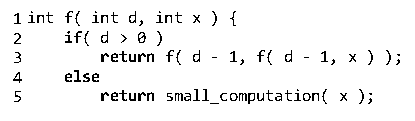
\includegraphics{Code/just_calling_benchmark}
\caption{The microbenchmark for measuring call frame allocation overhead.}
\label{fig:micro_calling}
\end{figure}

Most importantly, all the calls in the first version of this test were performed in yielding mode.
In atomic mode, calls and returns in \charcoal{} are just as efficient as plain C.
In well-tuned \charcoal{} code, most of the leaf and near-leaf calls should be performed in atomic mode.
To simulate this effect, we modified the benchmark to the version in Figure \ref{fig:micro_calling_n}.
The parameter \texttt{N} controls how deep in the call tree the benchmark uses yielding mode, before switching to atomic.

\vspace{1em}
\begin{tabular}{|l|r|r|r|}
  \hline
   & user & sys & wall \\
  \hline
  \hline
  Plain C & 0.77 & 0.00 & 0.77 \\
  \hline
  gcc split stacks\footnotemark{} & 1.00 & 0.15 & 1.15 \\
  \hline
  Go & 2.80 & 0.20 & 3.00 \\
  \hline
  Hot Stacking, \texttt{N} = 4 & 11.00 & 0.01 & 11.00 \\
  \hline
  Hot Stacking, \texttt{N} = 8 & 1.54 & 0.00 & 1.55 \\
  \hline
\end{tabular}
\vspace{1em}

\footnotetext{This benchmark does not create stacks deep enough to exceed the default size of a single segment of gcc's split stack.
So we modified the benchmark for the split stack case to make a linear chain of calls instead of a binary tree.}

This shows that with a modest fraction of the (static) calls performed in atomic mode, the calling overhead gets down to less than a factor of 2.
Combined with the observations above about tuning the language implementation, we believe this overhead would be barely noticeable for most applications.
Also it is worth noting that this is the price to be paid for the extremely low memory overhead of activities.

Hot stacking with \texttt{N} = 8 outperforms Go on this benchmark by a modest margin.
It is interesting that the gap between plain C and Go is as large as it is, given the Go implementation team's famous focus on low-level performance details.

gcc's split stack implementation outperforms hot stacking by a small margin on this benchmark.
However, as noted previously split stacks have bad performance in the pathological case where calls are made at high frequency right at the edge of a segment.

\begin{figure}
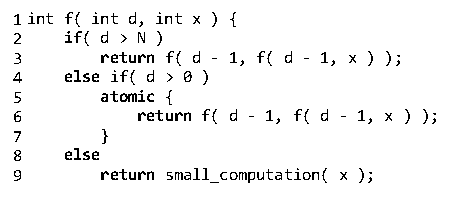
\includegraphics{Code/just_calling_n_benchmark}
\caption{The call/return microbenchmark modified to make some calls in atomic mode.}
\label{fig:micro_calling_n}
\end{figure}

\subsection{Yielding}

As described in section \ref{sec:yield_imp}, yield frequency can be managed fairly easily and the yield primitive is designed to have a very fast common path.
Nevertheless, it is important to minimize yielding in hot inner loops.

To quantify yielding overhead, we benchmarked a simple but problematic function from the C standard library: \texttt{strcmp}.
\texttt{strcmp} is tricky for a few reasons:
First, the input strings can be arbitrarily long, so never yielding could cause unresponsiveness.
Second, the body of the loop is extremely simple; good implementations are just a few assembly instructions.
This means that yielding every iteration causes significant performance overhead.
Third, the continued execution of the loop depends on the data read in each iteration, so simple loop tiling/blocking tricks do not work.
The best-performing implementation we have found so far appears in Figure \ref{fig:strcmp}.

\begin{figure}[htp]
\includegraphics[left]{Code/plain_strcmp}%
  \\
\includegraphics[left]{Code/strcmp_benchmark}%
\caption{Two implementations of \texttt{strcmp}.
  Top is a plain C version.
  Bottom is a \charcoal{} implementation aimed at minimizing yield overhead.}

\label{fig:strcmp}

\end{figure}


%% \begin{figure}
%%     \centering
%%     \begin{subfigure}[b]{0.3\textwidth}
%%         \hspace{-1.5cm}
%%         \includegraphics{plain_strcmp}
%%         \caption{}
%%     \end{subfigure}
%%     ~ %add desired spacing between images, e. g. ~, \quad, \qquad, \hfill etc. 
%%       %(or a blank line to force the subfigure onto a new line)
%%     \begin{subfigure}[b]{0.3\textwidth}
%%         \hspace{-1.5cm}
%%         \includegraphics{strcmp_benchmark}
%%         \caption{}
%%     \end{subfigure}
%%     \caption{Two implementations of \texttt{strcmp}.
%%       (a) is a plain C version.
%%       (b) is a \charcoal{} implementation aimed at minimizing yield overhead. }
%%     \label{fig:strcmp}
%% \end{figure}

In the code \texttt{YIELD\_FREQ} controls how frequently the loop yields.
The effect is that once every $2^{\mathtt{YF}}$ iterations there is a yield.

\vspace{1em}
\begin{tabular}{|l|r|}
  \hline
  Plain C & 430 \\
  \hline
  \charcoal, \texttt{YIELD\_FREQ = 4} & 1070 \\
  \hline
  \charcoal, \texttt{YIELD\_FREQ = 8} & 519 \\
  \hline
  \charcoal, \texttt{YIELD\_FREQ = 12} & 446 \\
  \hline
\end{tabular}
\vspace{1em}

These numbers are in microseconds per \texttt{strcmp} of two identical strings of 1MB length.
These data show that yielding is not free, but with a little careful tuning the yield overhead can be brought quite low.

When the inputs to \texttt{strcmp} are known to be short, the caller can wrap the call in atomic.
The atomic version should perform identically to the plain C implementation.

% \subsection{Code Size}

\subsection{Microbenchmark Summary}

Like all well implemented coroutines, the \charcoal{} implementation has extremely low memory and time overhead for basic concurrency primitives.
Hot stacking and frequent yielding are potential performance issues, but our tests indicate that at these overheads can be managed.

Though we do not have experience with writing large programs in \charcoal{} yet, we expect that relatively little code will require the kinds of contortions shown in the \texttt{strcmp} example.
Moreover, almost all such code will be in tight inner loops in library code.
This is exactly where writing somewhat weird code for performance reasons is acceptable.

%% \section{Foreign Code}

%% Foreign code (including legacy code) will never yield.  This could lead
%% to starvation pretty easily.  Here are three strategies:

%% \begin{itemize}
%% \item Do nothing.
%%   Just run the foreign code.
%%   This is a perfectly reasonable strategy as long as the foreign code does not run for a long time.
%% \item Run the foreign code in its own thread.
%%   If it has not returned by the end of some time slice, pause it to allow other activities to run.
%%   This runs the risk of creating atomicity violations galore.
%%   It also reintroduces the possibility of data races.
%%   However, it might be a reasonable strategy in situations where there is very little sharing between the foreign code and the rest of the application.
%% \item Run the foreign code in its own thread, but only interrupt it at special ``safe-ish'' points, like system calls.
%%   This is a compromise between the previous two strategies in the sense that it opens the door to both starvation and atomicity violations, but provides some (imperfect) protection against both.
%% \end{itemize}

%% We have not thought at all about what the best default is or what syntactic sugar would be nice.

%% Another important implementation issue to consider is foreign code that calls back in to activity-aware code.
%% There will definitely be some fancy footwork necessary there, no matter which strategy is used.

\section{Related Work}

Our activities are clearly closely related to many flavors of cooperative threads.
Most commonly, cooperative threads rely on programs explicitly invoking yield to permit task switching.
We believe that automatically inserting yields before and after calls by default creates a more predictable environment for programmers.
Boudol proposes a slightly different approach to automatic yield insertion in cooperative threads \cite{Boudol2007}.

The other major difference is the atomic block, which this paper shows is not a trivial addition to a language.
We are not aware of any other research on the combination of cooperative threads and atomic blocks.

One weakness that activities share with most multitasking frameworks is that activities cannot easily be run in parallel.
The authors are not optimistic about running cooperative threads in parallel, but there are researchers pursuing this idea \cite{ONeill2015, Boussinot2006, Dabrowski2006}.


%% Threads are the only multitasking abstractions discussed in this paper that naturally allow the parallel execution of tasks.
%% The authors view this as closer to a bug than a feature.
%% Serial multitasking abstractions like events and coroutines (and activities) can be used in combination with parallelism frameworks like processes and threads.
%% The authors consider providing both parallelism and multitasking in a single language features (like threads) mostly a bad idea.
%% Nevertheless, in the discussion section at the end of this paper we speculate about the feasibility of running activities in parallel.


% Threads without the Pain

%% \textbf{Hybrids}.
%% Researchers have long understood the weaknesses of existing multitasking abstractions.
%% Many proposals have been made for event/thread hybrids; for example: \cite{Boudol2007, Boussinot2006, Cunningham2005, Dabrowski2006, Fischer2007, Kerneis2014, Krohn2007, Li2007, Behren2003}.
%% A detailed comparison with all of these proposals is beyond the scope of this paper.
%% In the related work section we highlight the differences with the ones that are most similar to ours.


\section{Summary and Discussion}

In this paper we presented evidence that web applications seem to be highly exposed to atomicity violations.
We note that adding an atomic block would help programmers avoid these problems, and discussed how that addition can be achieved.
Perhaps the most important slogan to take from this paper is that the atomic versus async decision should be made by callers, not implementers of APIs.
We showed that our design can be implemented efficiently in a dialect of C.
We believe that our design combines the benefits of existing cooperative concurrency frameworks in a new and interesting way.


%% Acknowledgments
%% \begin{acks}                            %% acks environment is optional
%%                                         %% contents suppressed with 'anonymous'
%%   %% Commands \grantsponsor{<sponsorID>}{<name>}{<url>} and
%%   %% \grantnum[<url>]{<sponsorID>}{<number>} should be used to
%%   %% acknowledge financial support and will be used by metadata
%%   %% extraction tools.
%%   This material is based upon work supported by the
%%   \grantsponsor{GS100000001}{National Science
%%     Foundation}{http://dx.doi.org/10.13039/100000001} under Grant
%%   No.~\grantnum{GS100000001}{nnnnnnn} and Grant
%%   No.~\grantnum{GS100000001}{mmmmmmm}.  Any opinions, findings, and
%%   conclusions or recommendations expressed in this material are those
%%   of the author and do not necessarily reflect the views of the
%%   National Science Foundation.
%% \end{acks}




% We recommend abbrvnat bibliography style.

% \bibliographystyle{abbrvnat}
% \bibliographystyle{abbrv}

% The bibliography should be embedded for final submission.

\bibliography{./charcoal.bib}

%% \begin{thebibliography}{../../../../Documents/PapersForReferencing/biy_all_research.bib}
%% \softraggedright

%% \end{thebibliography}

\end{document}
